%Author: Marco Miani
%SWAN (developed by SWAN group, TU Delft, The Netherlands) is a wave spectral numerical model.
%For Simlating WAves Nearshore, it is necessary to define spatial grids of
%physical dominant factors (wind friction, dissipation) as well as define a COMPUTATIONAL
%grid on which the model performs its (spectral) calculations: budgeting energy spectra over
%each cell of the (computational) grid. Grids might have different spatial resolution and extension.

\documentclass[12pt]{article}
\usepackage{tikz}
\usepackage{verbatim}

\begin{comment}
:Title: SWAN wave model

SWAN_ (developed by SWAN group, TU Delft, The Netherlands) is a wave spectral numerical model. For Simlating WAves Nearshore, it is necessary to define spatial grids of
physical dominant factors (wind friction, dissipation) as well as define a COMPUTATIONAL
grid on which the model performs its (spectral) calculations: budgeting energy spectra over
each cell of the (computational) grid. Grids might have different spatial resolution and extension.

.. _SWAN: http://vlm089.citg.tudelft.nl/swan/index.htm

\end{comment}
\usetikzlibrary{positioning}
\begin{document}
\pagestyle{empty}


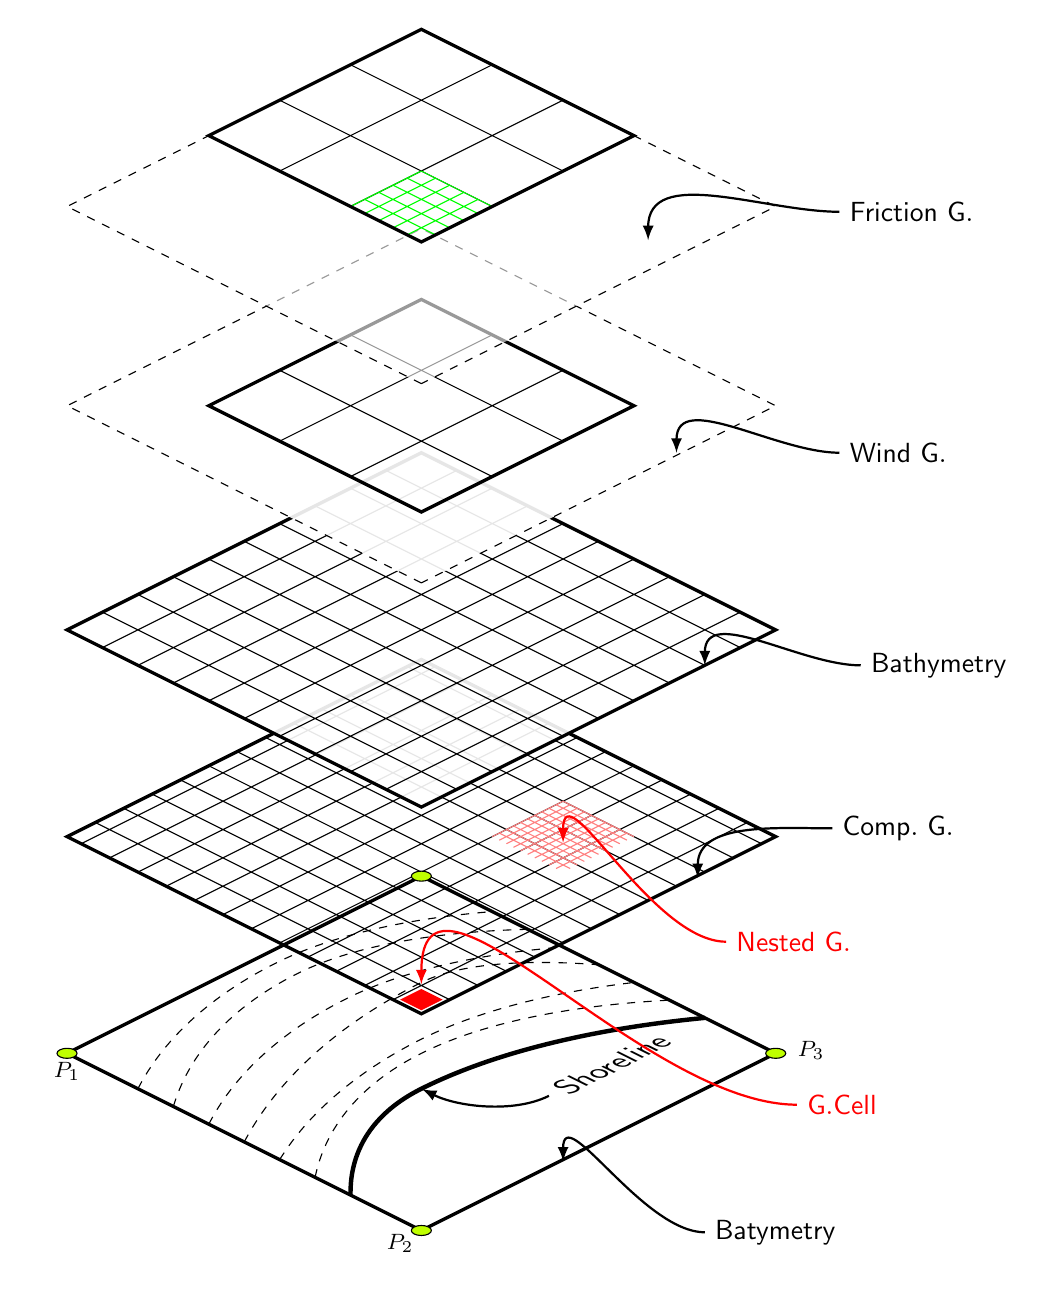
\begin{tikzpicture}[scale=.9,every node/.style={minimum size=1cm},on grid]
		
    %slanting: production of a set of n 'laminae' to be piled up. N=number of grids.
    \begin{scope}[
            yshift=-83,every node/.append style={
            yslant=0.5,xslant=-1},yslant=0.5,xslant=-1
            ]
        % opacity to prevent graphical interference
        \fill[white,fill opacity=0.9] (0,0) rectangle (5,5);
        \draw[step=4mm, black] (0,0) grid (5,5); %defining grids
        \draw[step=1mm, red!50,thin] (3,1) grid (4,2);  %Nested Grid
        \draw[black,very thick] (0,0) rectangle (5,5);%marking borders
        \fill[red] (0.05,0.05) rectangle (0.35,0.35);
        %Idem as above, for the n-th grid:
    \end{scope}
    	
    \begin{scope}[
    	yshift=0,every node/.append style={
    	    yslant=0.5,xslant=-1},yslant=0.5,xslant=-1
    	             ]
        \fill[white,fill opacity=.9] (0,0) rectangle (5,5);
        \draw[black,very thick] (0,0) rectangle (5,5);
        \draw[step=5mm, black] (0,0) grid (5,5);
    \end{scope}
    	
    \begin{scope}[
    	yshift=90,every node/.append style={
    	yslant=0.5,xslant=-1},yslant=0.5,xslant=-1
    	             ]
    	\fill[white,fill opacity=.9] (0,0) rectangle (5,5);
    	\draw[step=10mm, black] (1,1) grid (4,4);
    	\draw[black,very thick] (1,1) rectangle (4,4);
    	\draw[black,dashed] (0,0) rectangle (5,5);
    \end{scope}
    	
    \begin{scope}[
    	yshift=170,every node/.append style={
    	    yslant=0.5,xslant=-1},yslant=0.5,xslant=-1
    	  ]
        \fill[white,fill opacity=0.6] (0,0) rectangle (5,5);
        \draw[step=10mm, black] (2,2) grid (5,5);
        \draw[step=2mm, green] (2,2) grid (3,3);
        \draw[black,very thick] (2,2) rectangle (5,5);
        \draw[black,dashed] (0,0) rectangle (5,5);
    \end{scope}
    	
    \begin{scope}[
        yshift=-170,every node/.append style={
        yslant=0.5,xslant=-1},yslant=0.5,xslant=-1
                  ]
        %marking border
        \draw[black,very thick] (0,0) rectangle (5,5);

       	%drawing corners (P1,P2, P3): only 3 points needed to define a plane.
        \draw [fill=lime](0,0) circle (.1) ;
        \draw [fill=lime](0,5) circle (.1);
        \draw [fill=lime](5,0) circle (.1);
        \draw [fill=lime](5,5) circle (.1);

        %drawing bathymetric hypotetic countours on the bottom grid:    	
        \draw [ultra thick](0,1) parabola bend (2,2) (5,1)  ;
        \draw [dashed] (0,1.5) parabola bend (2.5,2.5) (5,1.5) ;
        \draw [dashed] (0,2) parabola bend (2.7,2.7) (5,2)  ;
        \draw [dashed] (0,2.5) parabola bend (3.5,3.5) (5,2.5)  ;
        \draw [dashed] (0,3.5)  parabola bend (2.75,4.5) (5,3.5);
        \draw [dashed] (0,4)  parabola bend (2.75,4.8) (5,4);
        \draw [dashed] (0,3)  parabola bend (2.75,3.8) (5,3);
        \draw[-latex,thick](2.8,1)node[right]{$\mathsf{Shoreline}$}
                 to[out=180,in=270] (2,1.99);
    \end{scope} %end of drawing grids

    %putting arrows and labels:
    \draw[-latex,thick] (6.2,2) node[right]{$\mathsf{Bathymetry}$}
         to[out=180,in=90] (4,2);

    \draw[-latex,thick](5.8,-.3)node[right]{$\mathsf{Comp.\ G.}$}
        to[out=180,in=90] (3.9,-1);

    \draw[-latex,thick](5.9,5)node[right]{$\mathsf{Wind\ G.}$}
        to[out=180,in=90] (3.6,5);

    \draw[-latex,thick](5.9,8.4)node[right]{$\mathsf{Friction\ G.}$}
        to[out=180,in=90] (3.2,8);

    \draw[-latex,thick,red](5.3,-4.2)node[right]{$\mathsf{G. Cell}$}
        to[out=180,in=90] (0,-2.5);

    \draw[-latex,thick,red](4.3,-1.9)node[right]{$\mathsf{Nested\ G.}$}
        to[out=180,in=90] (2,-.5);

    \draw[-latex,thick](4,-6)node[right]{$\mathsf{Batymetry}$}
        to[out=180,in=90] (2,-5);	
    %drawing points on grid's conrners.
    \fill[black,font=\footnotesize]
        (-5,-4.3) node [above] {$P_{1}$}
        (-.3,-5.6) node [below] {$P_{2}$}
        (5.5,-4) node [above] {$P_{3}$};	
\end{tikzpicture}

\end{document} 